\section{Evaluation}

\begin{frame}
    \frametitle{Counting crates with UB}
    \begin{figure}
        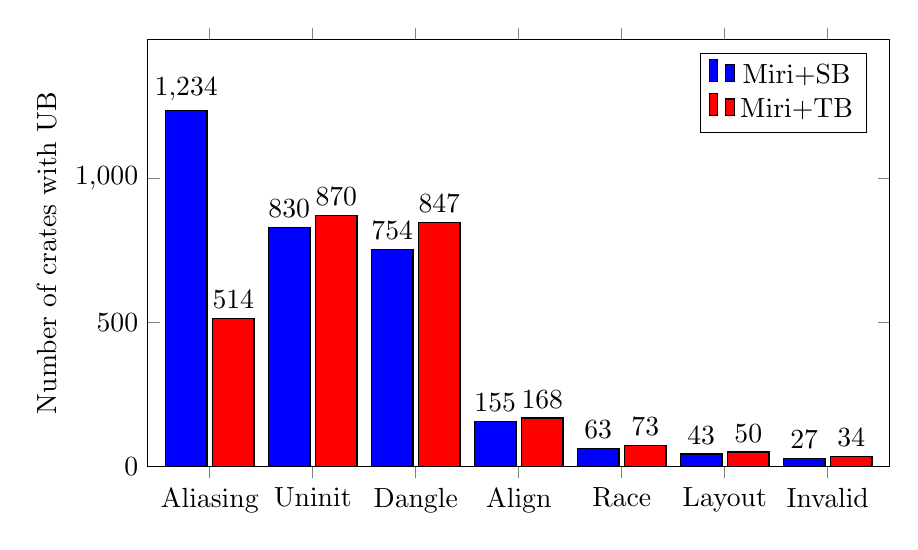
\begin{tikzpicture}
            \begin{axis}[
                    ybar,
                    ymin=0,
                    width=11cm,
                    height=7cm,
                    bar width=15pt,
                    ylabel={Number of crates with UB},
                    nodes near coords,
             %      nodes near coords align=below, % places labels inside bars
                    symbolic x coords={Aliasing, Uninit, Dangle, Align, Race, Layout, Invalid},
                    xtick = data,
                    enlarge y limits={value=0.2,upper},
                    legend pos=north east
                ]
                \addplot[fill=blue] coordinates {(Aliasing, 1234) (Uninit, 830) (Dangle, 754) (Align, 155) (Race, 63) (Layout, 43) (Invalid, 27)};
                \addplot[fill=red] coordinates {(Aliasing, 514) (Uninit, 870) (Dangle, 847) (Align, 168) (Race, 73) (Layout, 50) (Invalid, 34)};
                \legend{Miri+SB,Miri+TB}
            \end{axis}
        \end{tikzpicture}
    \end{figure}
\end{frame}

\begin{frame}
    \frametitle{Summary}
    \begin{itemize}
        \item Tree Borrows UB is much less common on \texttt{crates.io} than Stacked Borrows UB\\
            \(\qquad\Rightarrow\) fulfills goal of being more permissive
            \begin{block}{Notable examples}
                \texttt{tokio}, \texttt{pyo3}, \texttt{rkyv}, \texttt{eyre}, \texttt{ndarray}, ...\\
                \texttt{arrayvec}, \texttt{slotmap}, \texttt{nalgebra}, \texttt{json}, ...\\
            \end{block}
        \item patterns allowed by Stacked Borrows but forbidden by Tree Borrows are theoretically
            possible but rare
            \begin{itemize}
                \item TB has existed for one year, no complaint about those yet
            \end{itemize}
    \end{itemize}
\end{frame}

\begin{frame}
    \frametitle{Summary}
    \begin{itemize}
        \item Tree Borrows UB is much less common on \texttt{crates.io} than Stacked Borrows UB\\
            \(\qquad\Rightarrow\) fulfills goal of being more permissive
        \item elimination of out-of-bounds UB\\
            \(\qquad\Rightarrow\) blocker in SB for many popular crates
        \item patterns allowed by Stacked Borrows but forbidden by Tree Borrows are rare
    \end{itemize}
\end{frame}

\begin{frame}
    \frametitle{Questions ?}

    TB also has...
    \begin{itemize}
        \item tweaked rules for interactions between interior mutability and protectors/\texttt{Reserved}
        \item performance improvements compared to the naive implementation
            \begin{itemize}
                \item many tricks to trim tree traversals
                \item lazy initialization for out-of-range accesses
            \end{itemize}
        \item ongoing attempt at formalization in Coq
    \end{itemize}~\\~\\
    \vfill

    Don't hesitate to test your code with Miri and send us your interesting/unexpected cases of UB!\\
    Slides and examples on \href{https://github.com/Vanille-N/tree-beamer/tree/ens}{\texttt{github:Vanille-N/tree-beamer/tree/ens}}\\
    Complementary material: \href{https://perso.crans.org/vanille/treebor}{\texttt{perso.crans.org/vanille/treebor}}\\
\end{frame}
